\section{基本的な定義}

\setcolumnwidth{0.8\textwidth, 0.2\textwidth}
\begin{paracol}{2}
\paragraph{グラフの頂点集合と辺集合}
グラフ$G=(V, E)$は有限集合$V$と
$V$の直積の部分集合$E \subseteq V\times V$の二個組からなる組合せ構造である。
集合$S$と$T$の直積は$S$と$T$から要素を
それぞれ一つ取り出して形成するペアを全て集めて作った集合で$S\times T$と書く。
平面の座標空間を${\mathbb R}^2$と書くように、
集合$V$の直積は$V\times V$を省略して$V^2$と書くこともある。
$V$の要素を頂点、$E$の要素を辺と呼ぶ。
これらの名称は多角形・多面体に倣う。
各辺に順序が付与され系列として扱う場合$G$を有向グラフという。
そうでない場合は無向グラフという。
辺$(u, v)$の頂点$u, v$を端点という。
有向グラフにおいては$u$を始点$v$を終点と呼ぶ。
\switchcolumn
\vspace{-0.5\intextsep}
\begin{figure}[ht]
\centering
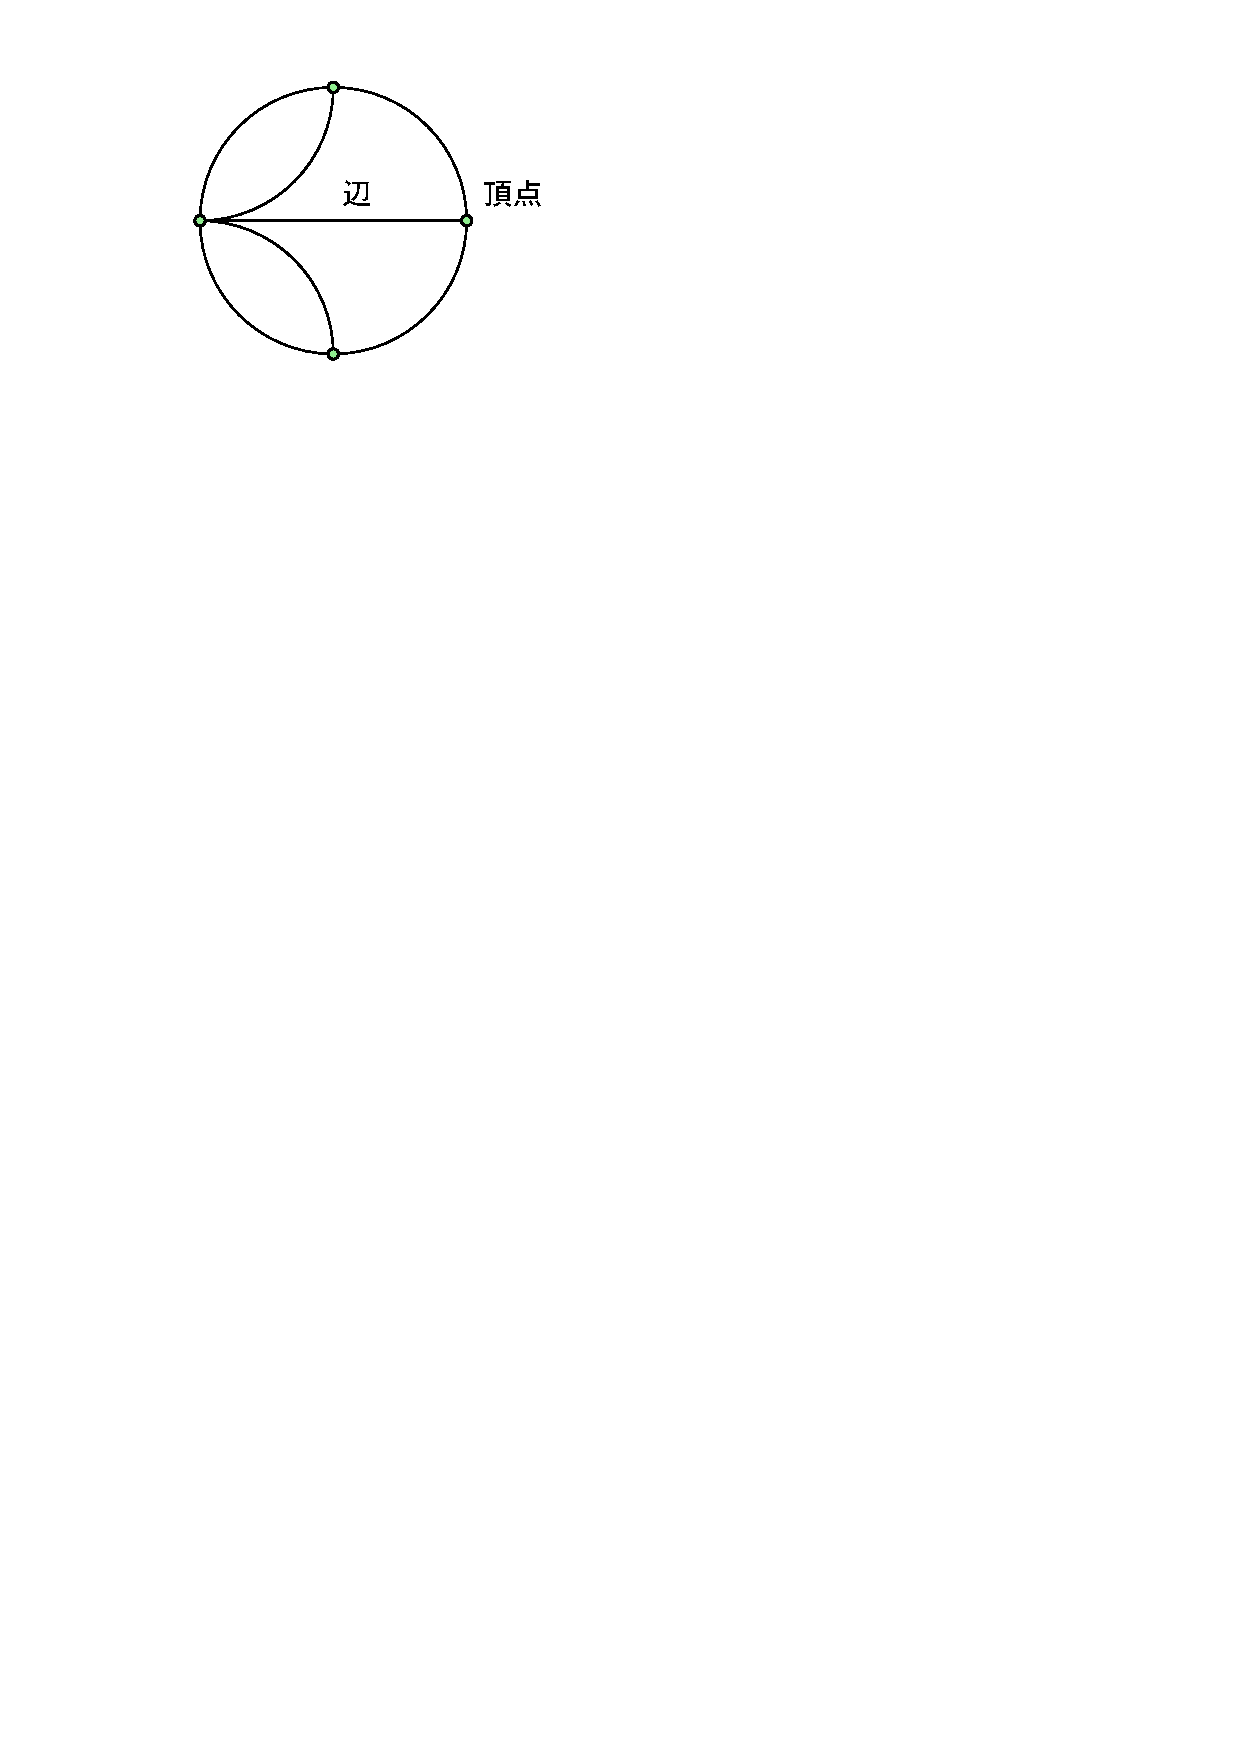
\includegraphics[width=0.15\textwidth]{figures/Konigsberg.pdf}\\
{\small ケーニヒスベルクの\\七つの橋}
\end{figure}
\end{paracol}




\setcolumnwidth{0.9\textwidth, 0.1\textwidth}
\begin{paracol}{2}
\paragraph{単純グラフ}
ある辺$e=(u, v)$が$u=v$の場合$e$を自己ループという。
グラフ$G=(V, E)$が単純であるという言及は、
$E$に自己ループや重複する辺を含まないことを意味する。
重複する辺を許す場合、それらの辺を多重辺と呼ぶ。
平面性を判定する際は、
自己ループや多重辺を削除もしくは細分した単純なグラフを対象とする。
\switchcolumn
%\vspace{-0.5\intextsep}
\begin{figure}[ht]
\centering
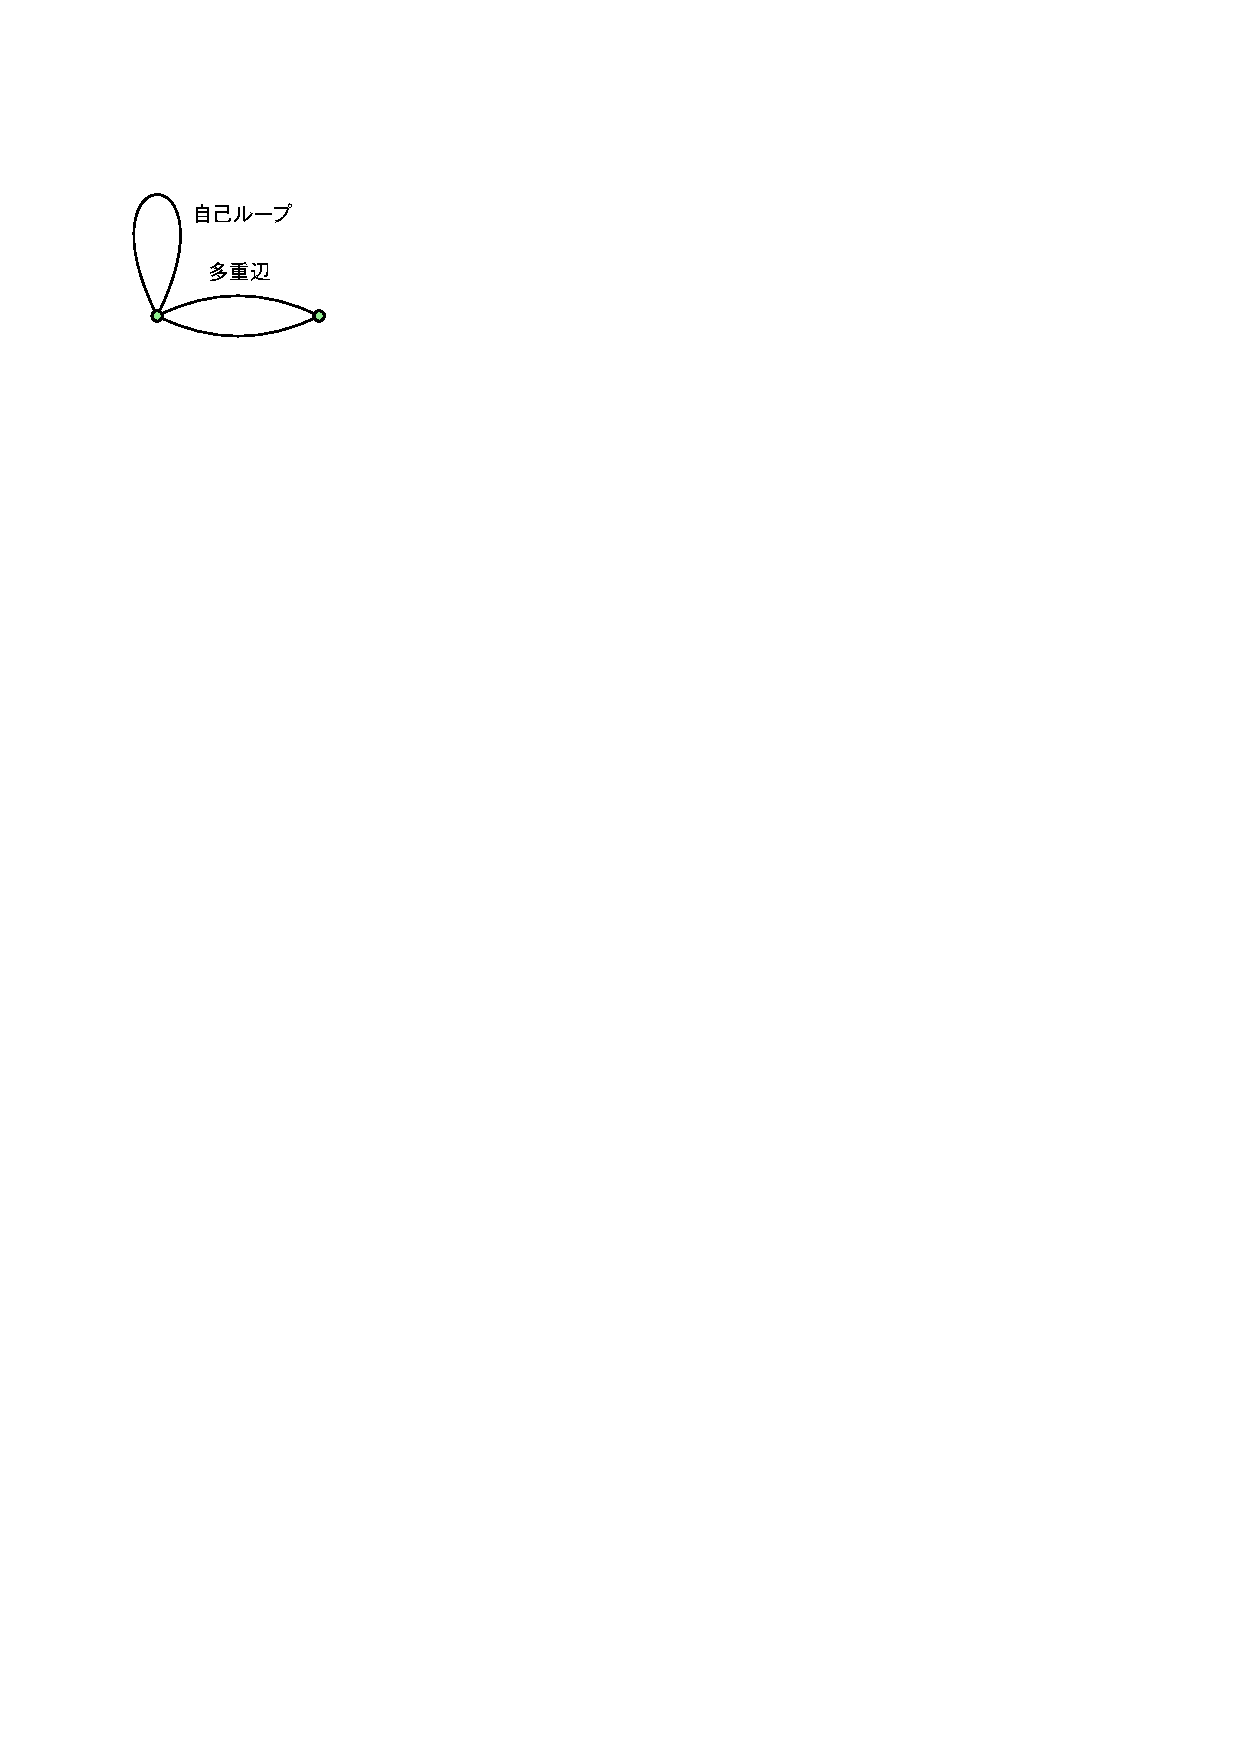
\includegraphics[width=0.09\textwidth]{figures/self_loop_and_multiedges.pdf}
\end{figure}
\end{paracol}


\setcolumnwidth{0.85\textwidth, 0.15\textwidth}
\begin{paracol}{2}
\paragraph{頂点と辺の近接性}
無向グラフ$G=(V, E)$において$e=(u, v)\in E$なら$u$と$v$は互いに隣接するという。
また、$e$は$u$と$v$を接続するという。
頂点$u$の隣接頂点の集合$N(u)$は
%$N(u) = \{v \mathrm{\ for\ } (u, v) \in E\}$のように記述できる。
$N(u) = \{v ~|~ (u, v) \in E\}$のように記述できる。
頂点$v$の次数を$\deg(v)$と書き$v$に接続する辺の個数とする。
$\deg(v) = |N(v)|$とも書ける。
$\deg(v)=0$の頂点$v$を孤立点という。

\switchcolumn
\vspace{1.0\intextsep}
\begin{figure}[ht]
\centering
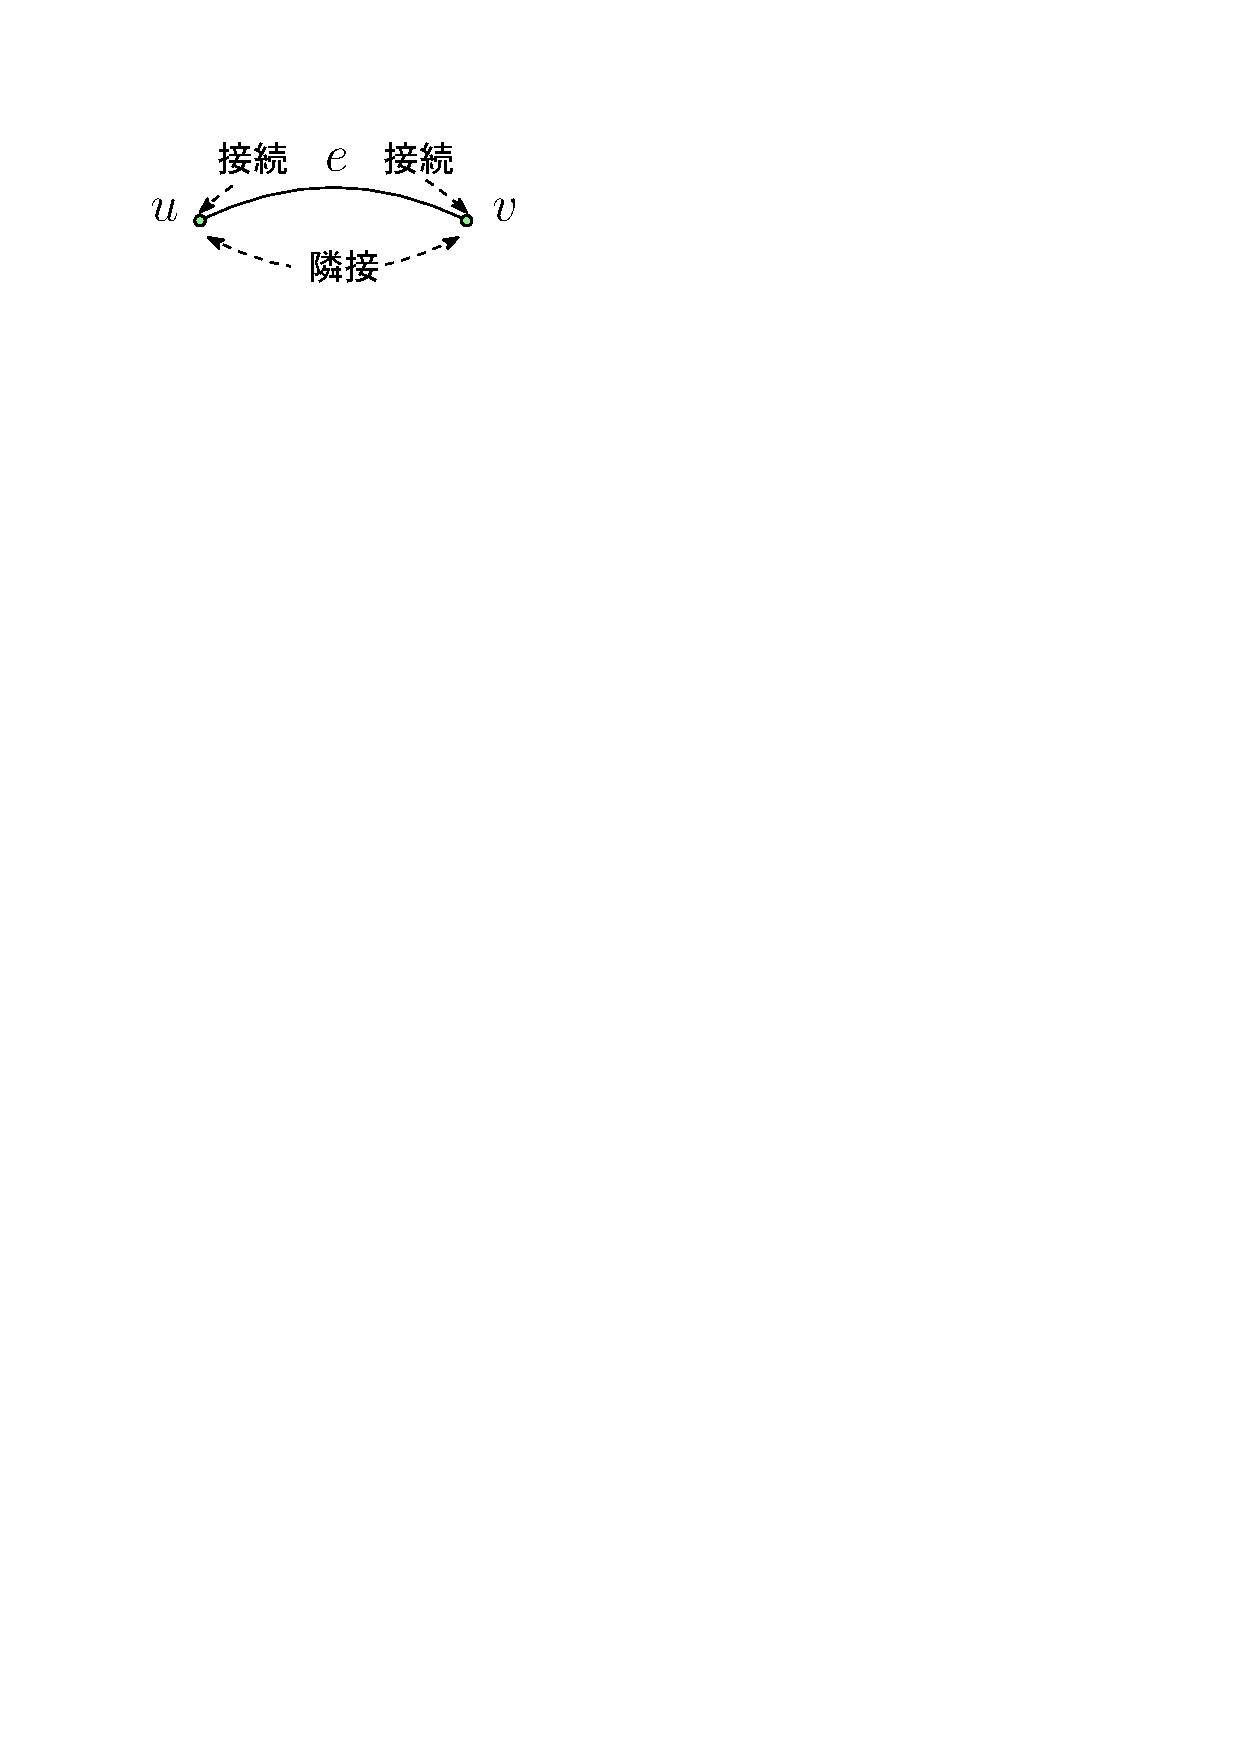
\includegraphics[width=0.14\textwidth]{figures/neighbors.pdf}
\end{figure}
\end{paracol}


\setcolumnwidth{0.8\textwidth, 0.2\textwidth}
\begin{paracol}{2}
\paragraph{完全グラフ}
すべての二頂点が隣接するグラフを完全グラフという。
つまり$G=(V, E)$に対して$E=V^2$。
$n$頂点の完全グラフを$K_n$と書く。
グラフ$G=(V_1 \cup V_2, E)$が、頂点集合を二つの互いに素な集合$V_1, V_2$に分割でき、
どの辺も$V_1$の頂点と$V_2$の頂点を接続するグラフを二部グラフという。
完全二部グラフはその辺集合が$E = V_1 \times V_2$となるグラフである。
$K_{n_1, n_2}$で$n_1, n_2 = |V_1|, |V_2|$の完全二部グラフを表す。
\switchcolumn
\vspace{0.5\intextsep}
\begin{figure}[ht]
\centering
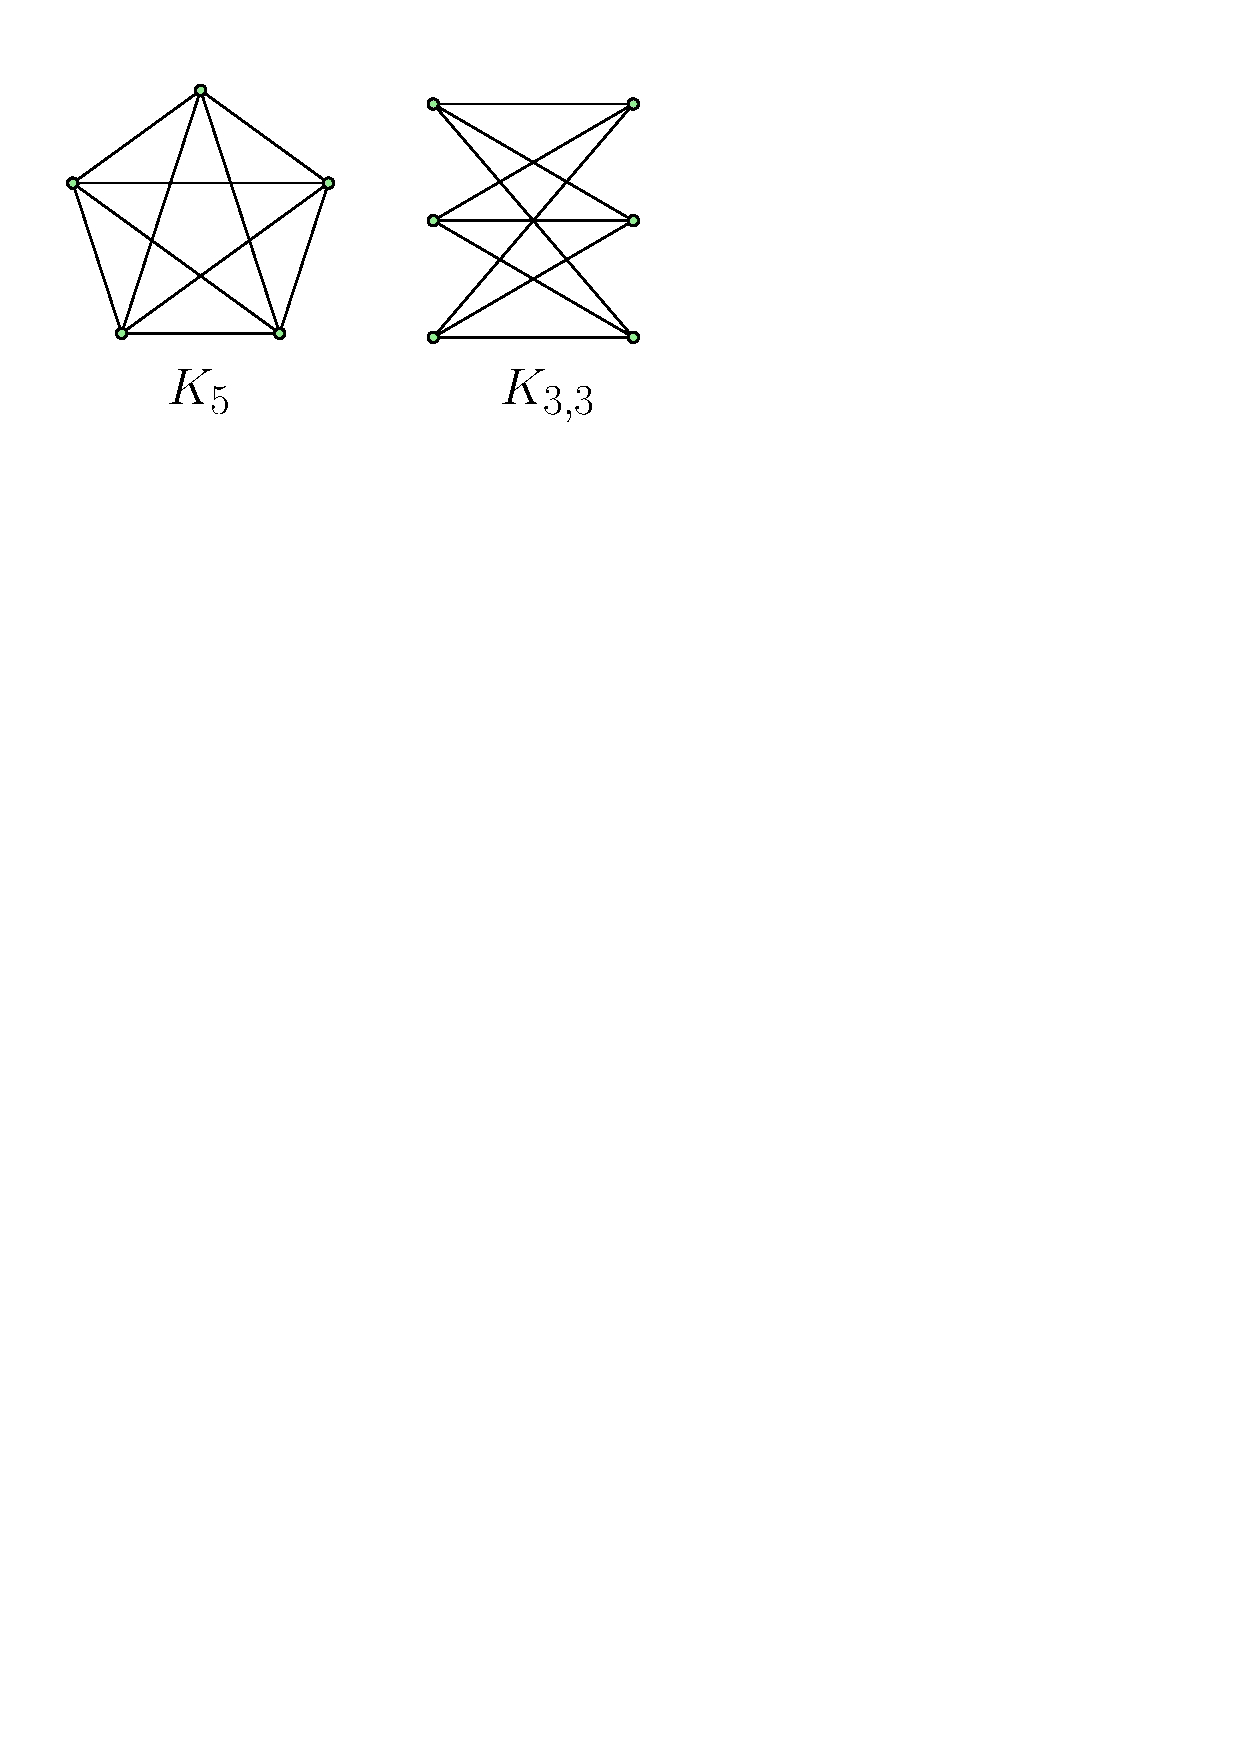
\includegraphics[width=0.19\textwidth]{figures/complete_graphs.pdf}
\end{figure}
\end{paracol}





%\vspace*{-0.7\intextsep}
\setcolumnwidth{0.7\textwidth, 0.3\textwidth}
\begin{paracol}{2}
\paragraph{グラフの局所編集(削除、縮約、細分)}
$G=(V, E)$からある辺$e \in E$を削除して得られるグラフを$G\setminus e$で表す。
$G\setminus e$は$e$以外の$G$の接続関係を継承する。
同様に$G\setminus v$で、
頂点$v\in V$と$v$に接続するすべての辺を削除することで得られるグラフを表わす。
二項演算子$\setminus$は集合の差演算に倣う。
また、
$S \subseteq V$や$T \subseteq E$に対して$G\setminus S$や$G\setminus T$の記述を許す。

辺$e$が自己ループや多重辺でないとき、
$e$の縮約は$e$の端点を併合して一つの頂点$v_e$としつつ$e$を削除する操作である。
このとき両端点に接続する$e$を除くすべての辺の接続関係を$v_e$に引き継ぐ。
自己ループや多重辺に縮約は適用できない。
$G / e$によって副次的に多重辺が生成されるが一般的にこれは削除され単純化される。
ただ、数学的帰納法など証明手順によっては敢えて多重辺を削除しないこともある。
$G / e$で$e$を縮約して得られるグラフを表す。
これも$T\subseteq E$に対して$G / T$のような記述を許す。

グラフの辺細分は、
ある一辺の内部を部分分割して二辺で置き換える操作である。
$K_{3,3}$もしくは$K_5$に対して有限回の辺細分を適用して得られるグラフを
クラトフスキーグラフという。
クラトフスキーグラフは、グラフの平面性を特徴付ける重要な役割を果たす。

\switchcolumn
\vspace{1.5\intextsep}
%\begin{figure}[ht]
\centering
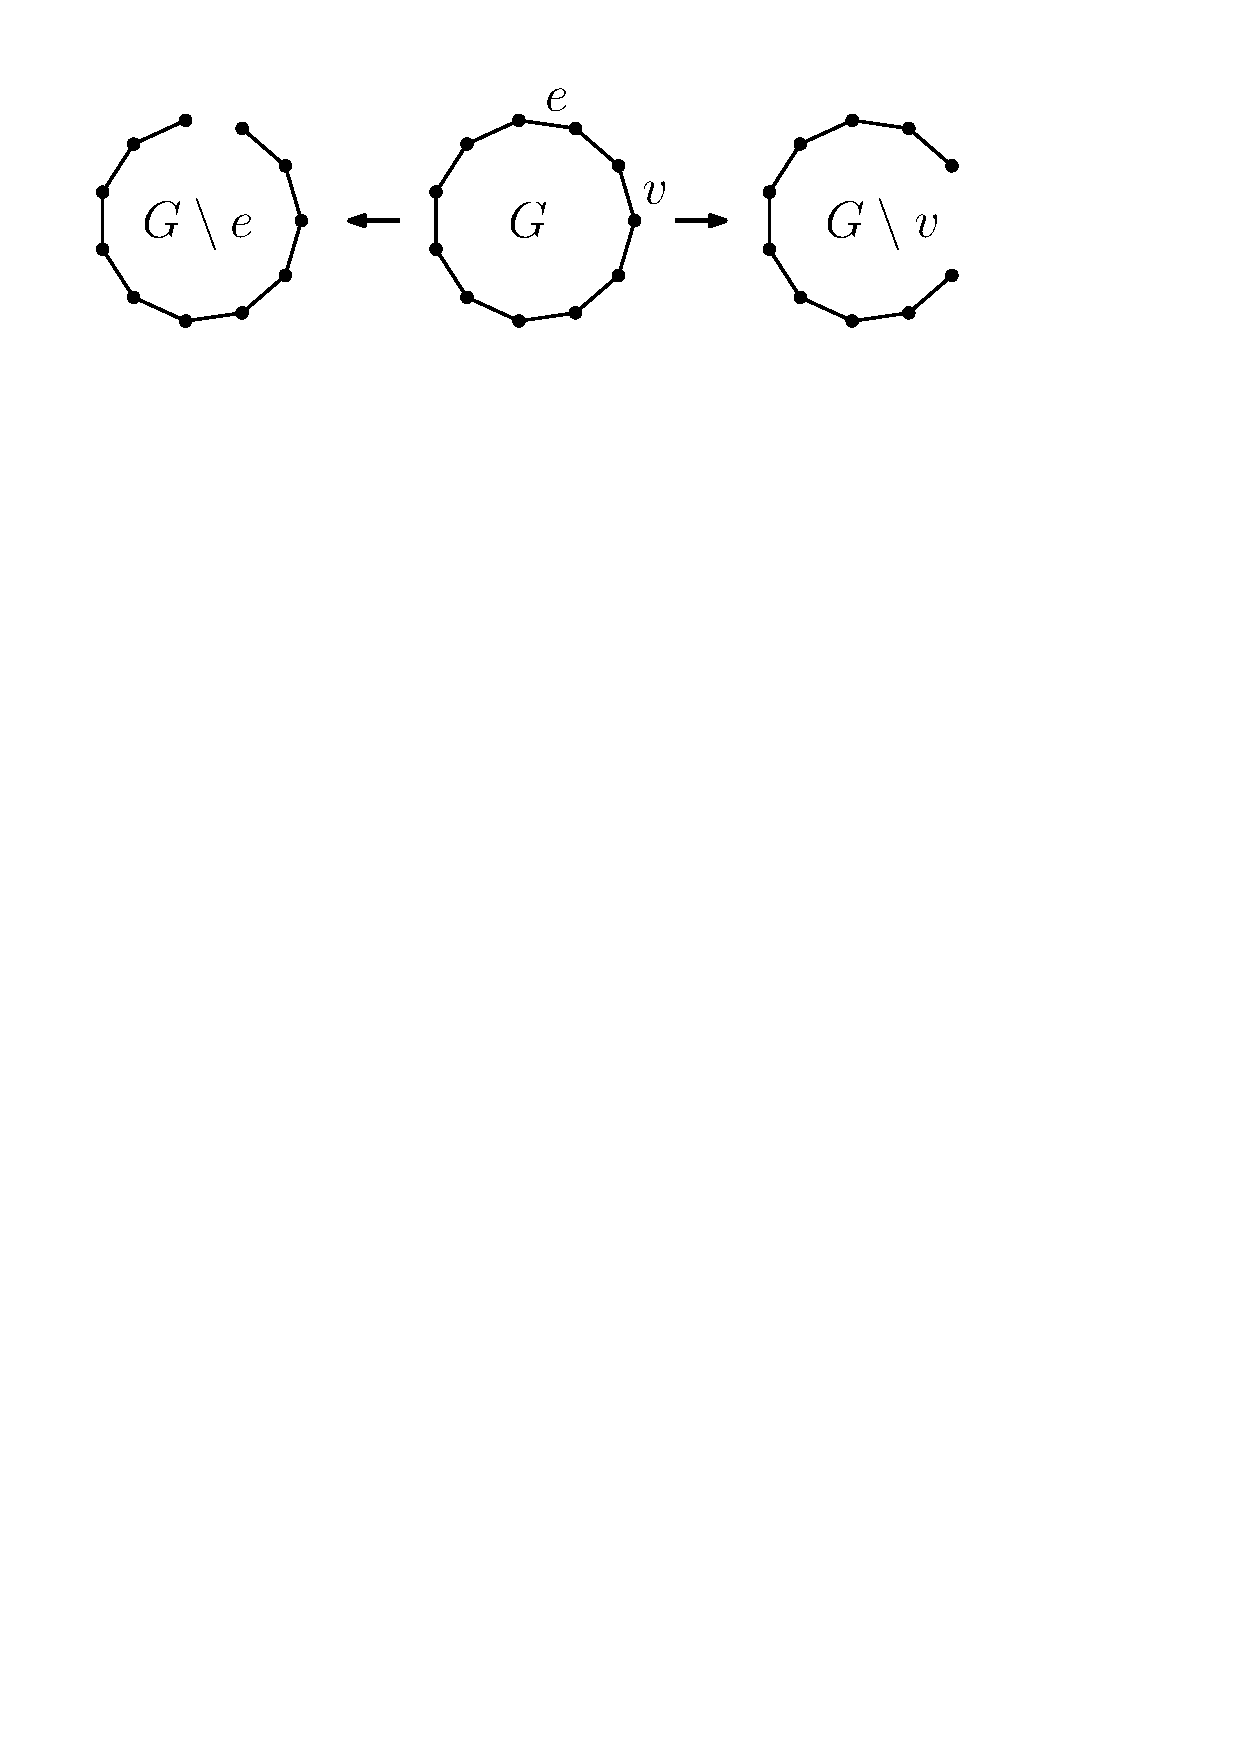
\includegraphics[width=0.29\textwidth]{figures/deleting.pdf}

\vspace{1.5\intextsep}
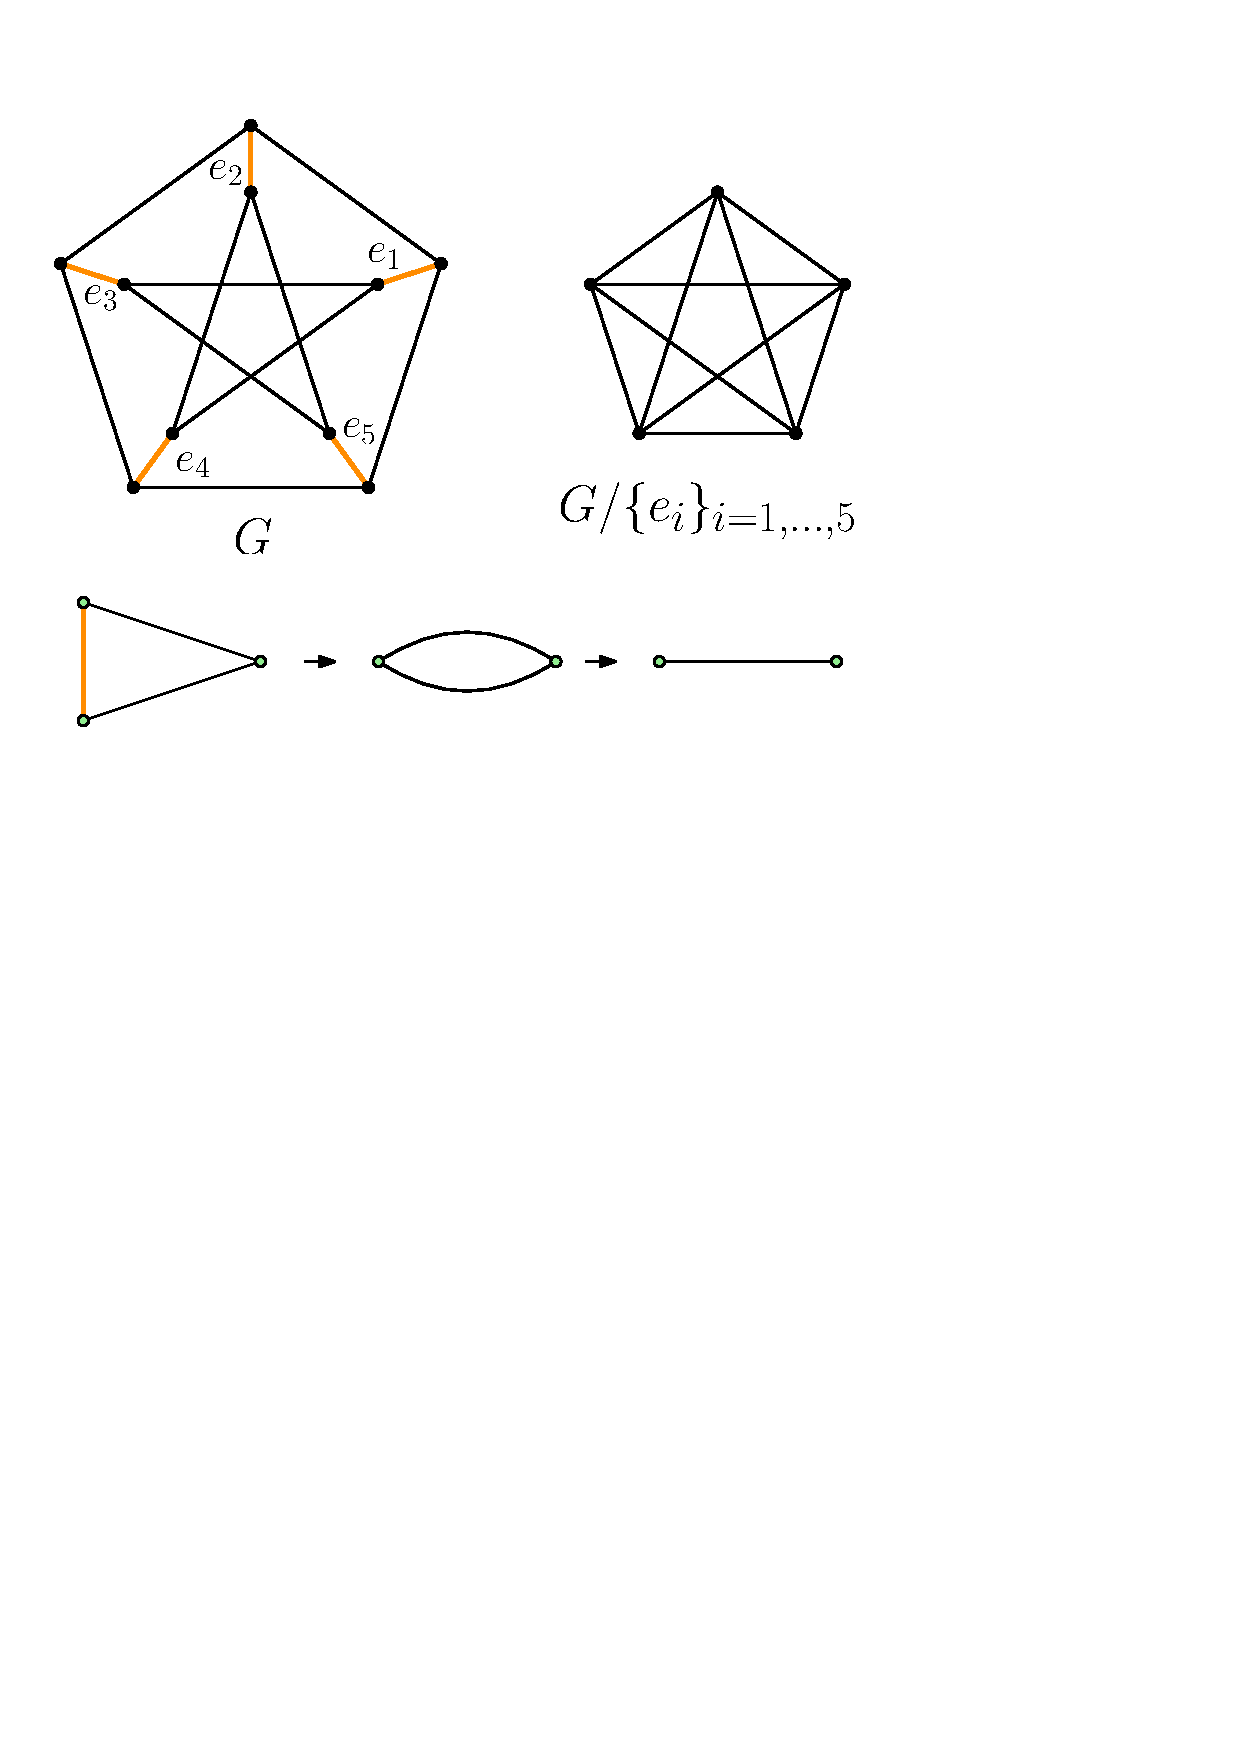
\includegraphics[width=0.20\textwidth]{figures/edge_contractions.pdf}

\vspace{1.\intextsep}
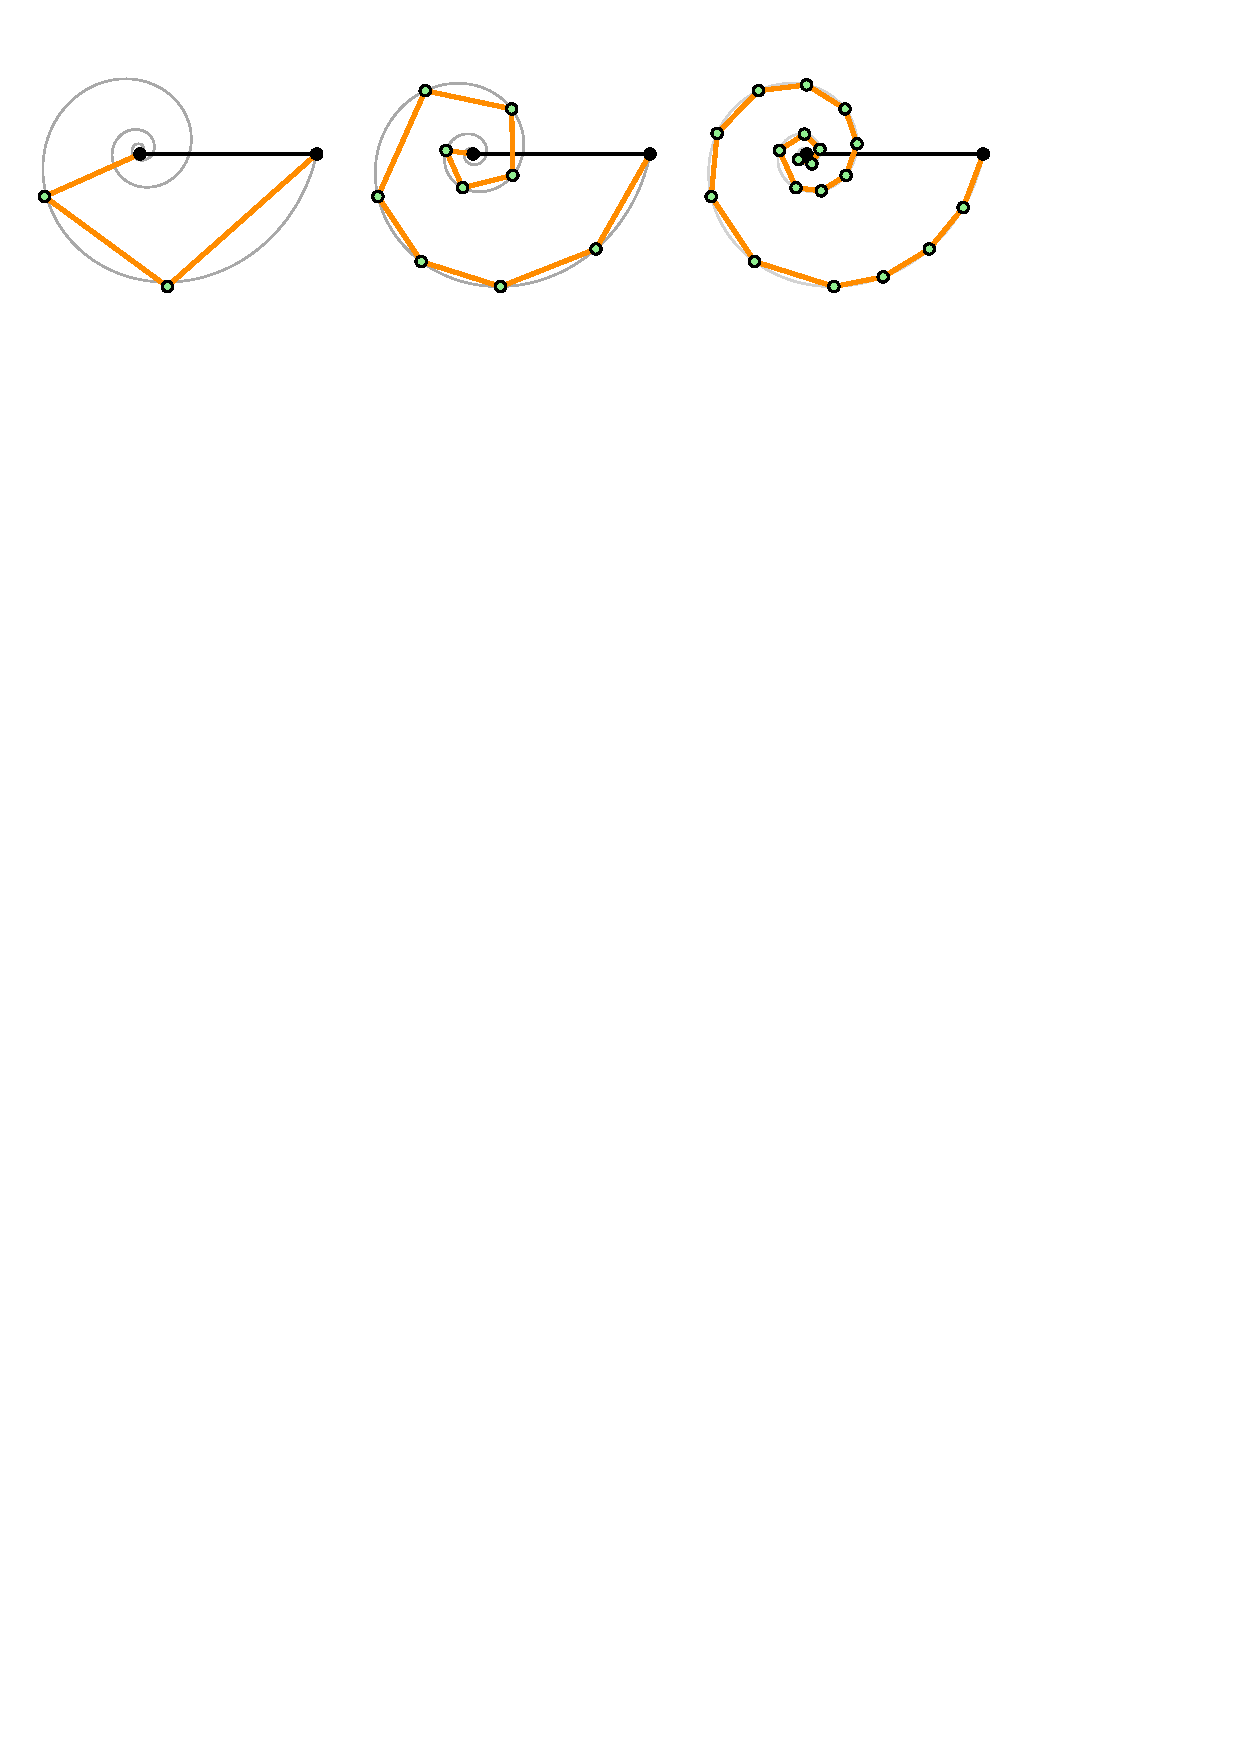
\includegraphics[width=0.29\textwidth]{figures/edge_subdivision.pdf}
%\end{figure}
\end{paracol}

\setcolumnwidth{0.7\textwidth, 0.3\textwidth}
\begin{paracol}{2}
\paragraph{グラフの集合演算と部分グラフ}
グラフ$G_1 = (V_1, E_1)$と$G_2=(V_2, E_2)$に対して
グラフの和を$G_1 \cup G_2 = (V_1 \cup V_2, E_1 \cup E_2)$とする。
同様にグラフの積を$G_1 \cap G_2 = (V_1 \cap V_2, E_1 \cap E_2)$とする。
あるグラフ$G$および$H$に対して$G \cup H = G$のとき$H$を$G$の部分グラフという。
任意の頂点集合$S \subseteq V$に対して、
頂点集合が$S$であり、辺集合が$E$の部分集合で両端点が$S$に含まれるものを
$G[S]$と書き$G$の誘導部分グラフという(右図右)。
また、任意の辺集合$T\subseteq E$が誘導するグラフ$G[T]$を
$G[T]=(V_T, T)$と定義する。
ただし$V_T=\bigcup\limits_{(x,y)\in T}\{x, y\}$。

\switchcolumn
%\vspace{1.5\intextsep}
\centering
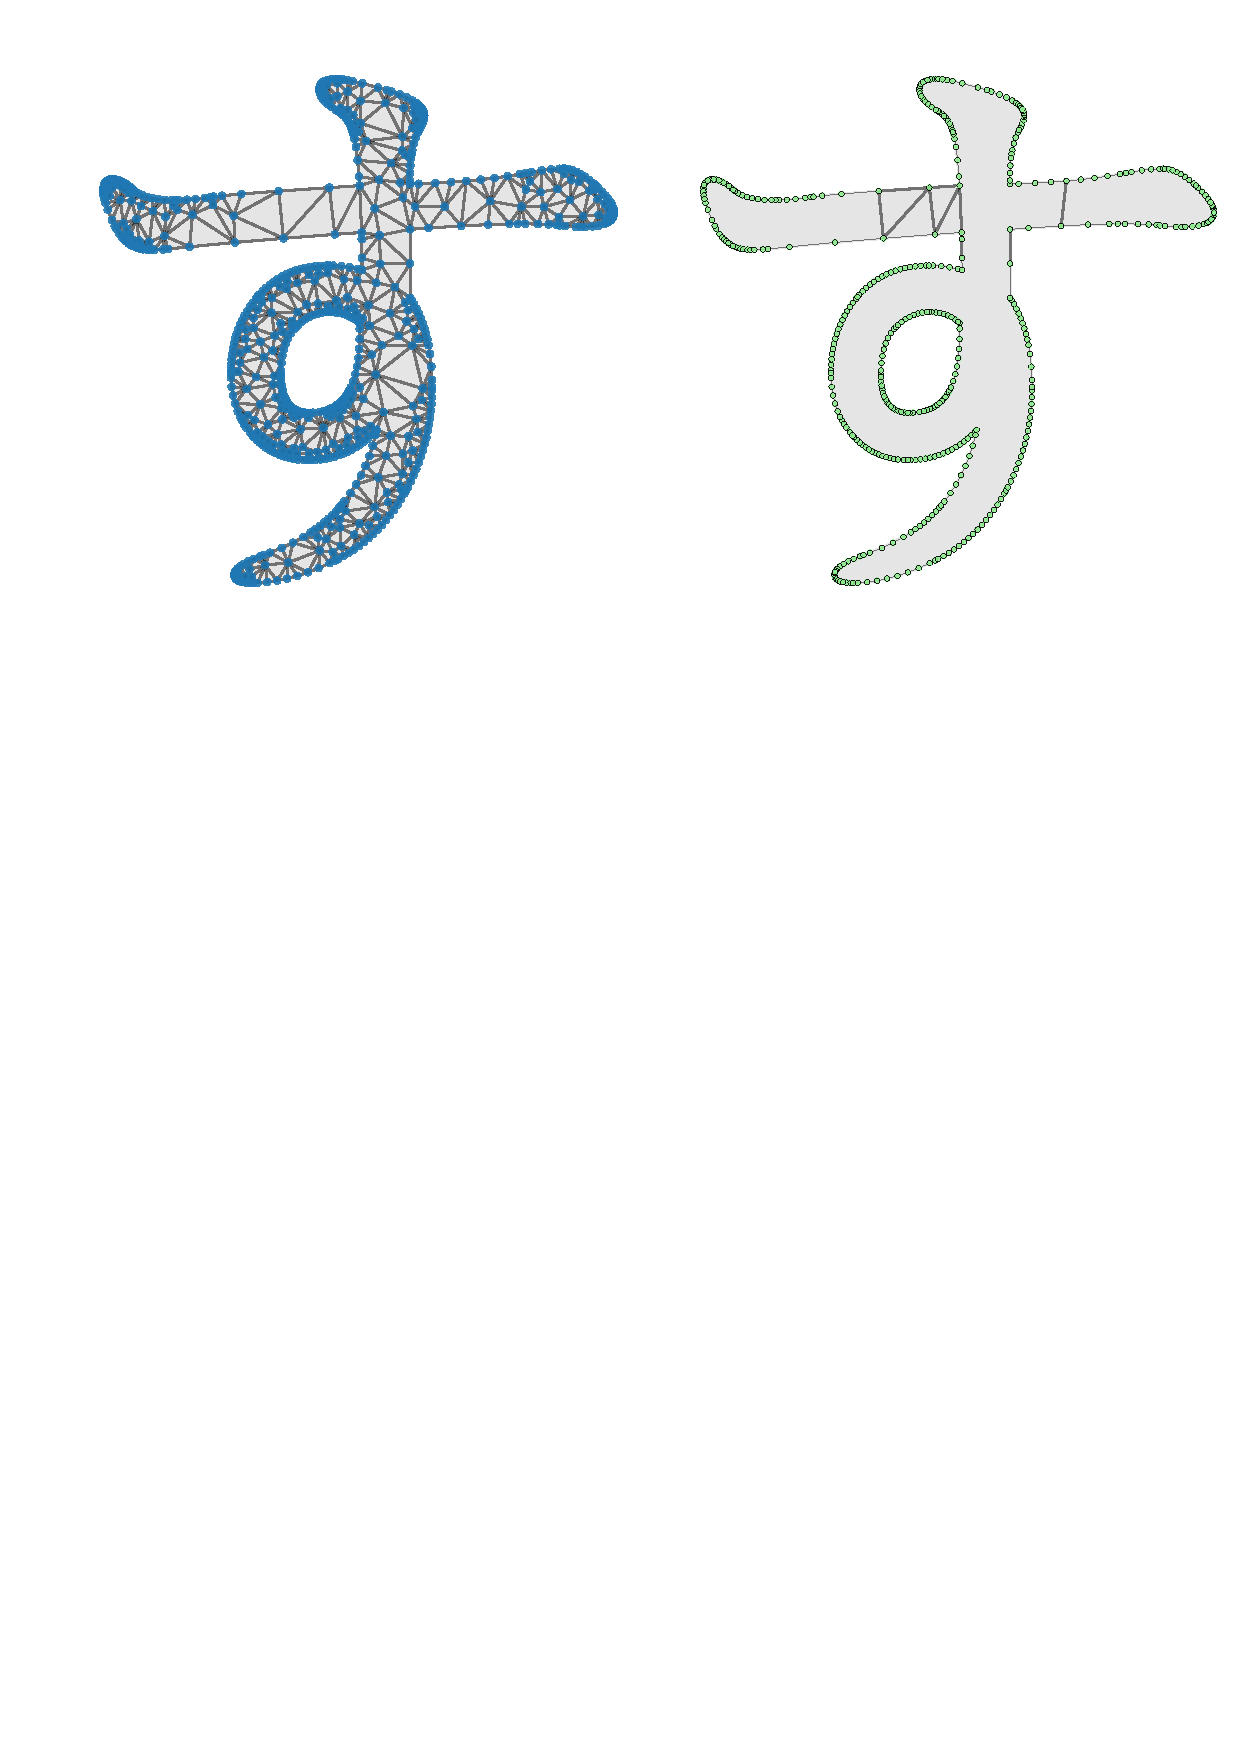
\includegraphics[width=0.29\textwidth]{figures/connect_su.pdf}

{\small ひらがな「す」のアウトラインの\\頂点集合を$S$とした際の
誘導部分グラフ$G[S]$。~~~~~~~~~~~~~~~~~~~~~~~~~}
\end{paracol}

\setcolumnwidth{0.85\textwidth, 0.15\textwidth}
\begin{paracol}{2}
\paragraph{経路と閉路}
次の条件を満たす頂点と辺の交互列を経路もしくはパスという。
始点と終点が異なる頂点で、
連続する頂点と辺は接続し、
いずれの頂点と辺も重複しない。
%始点と終点はそれぞれ交互列の先頭と末尾の頂点とする。
始点と終点が同じ経路を閉路という。
経路や閉路の長さは辺の個数で測られる。
一般的に任意の経路の長さは$1$以上だが
数学的帰納法を用いる証明手段や言語実装など、
頂点一つからなる長さ$0$の経路を許すと簡潔に記述できることがある。
無向グラフにおいて頂点$u, v$間に経路$p$が存在するなら、
$u$と$v$は互いに到達可能であるといい$p$は$u$と$v$を接続するという。
%同様に、有向グラフにおいては頂点$u$から$v$にパスが存在する場合
%$u$から$v$へ到達可能であるという。
グラフ内の最小閉路の長さを\hlpink{内周}という。
閉路を持たないグラフの内周は$\infty$とする。


\switchcolumn
\vspace{1.5\intextsep}
\centering
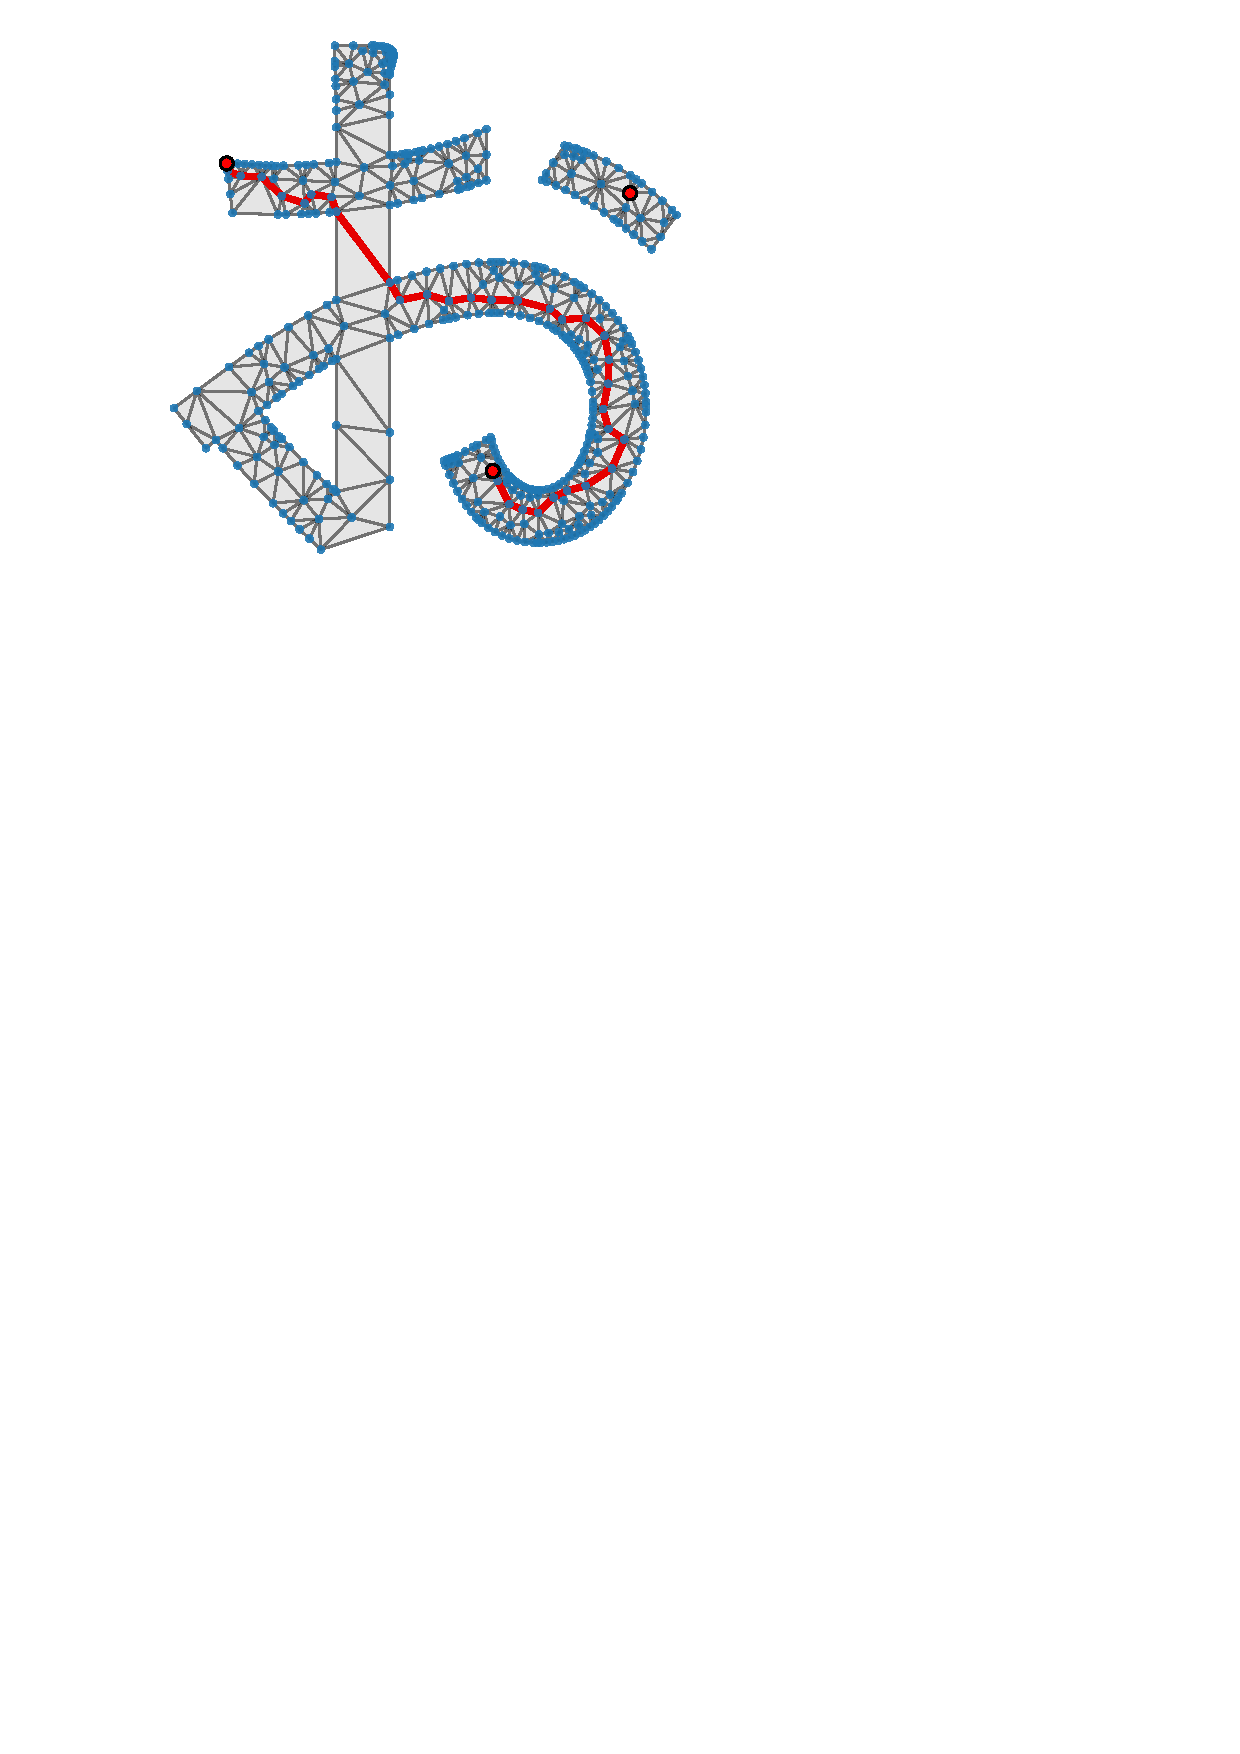
\includegraphics[width=0.14\textwidth]{figures/paths.pdf}
\end{paracol}




\setcolumnwidth{0.7\textwidth, 0.3\textwidth}
\begin{paracol}{2}
\paragraph{グラフの連結性}
無向グラフが\hlpink{連結}であるという言及は
任意の二頂点が互いに到達可能であることを意味する。
逆に互いに到達可能でない頂点対が一つでもあれば、そのグラフは\hlpink{非連結}であるという。
非連結なグラフ内の連結な部分グラフを\hlpink{連結成分}という。
ある頂点$v$をグラフから削除すると非連結になるとき$v$を\hlpink{切断点}という。
同様に、ある辺$e$の削除で非連結になるなら$e$を\hlpink{橋}という。
閉路を持たない連結なグラフを木という。
木における頂点および辺は、いずれも切断点であり、橋である。
平面性判定は連結成分ごとに実行すれば良いので、
%以下では断りが無い限り入力として与えられるグラフは連結グラフとする。
以下では対象グラフは連結とする。

\switchcolumn
%\begin{figure}[ht]
\vspace{1.5\intextsep}
\centering
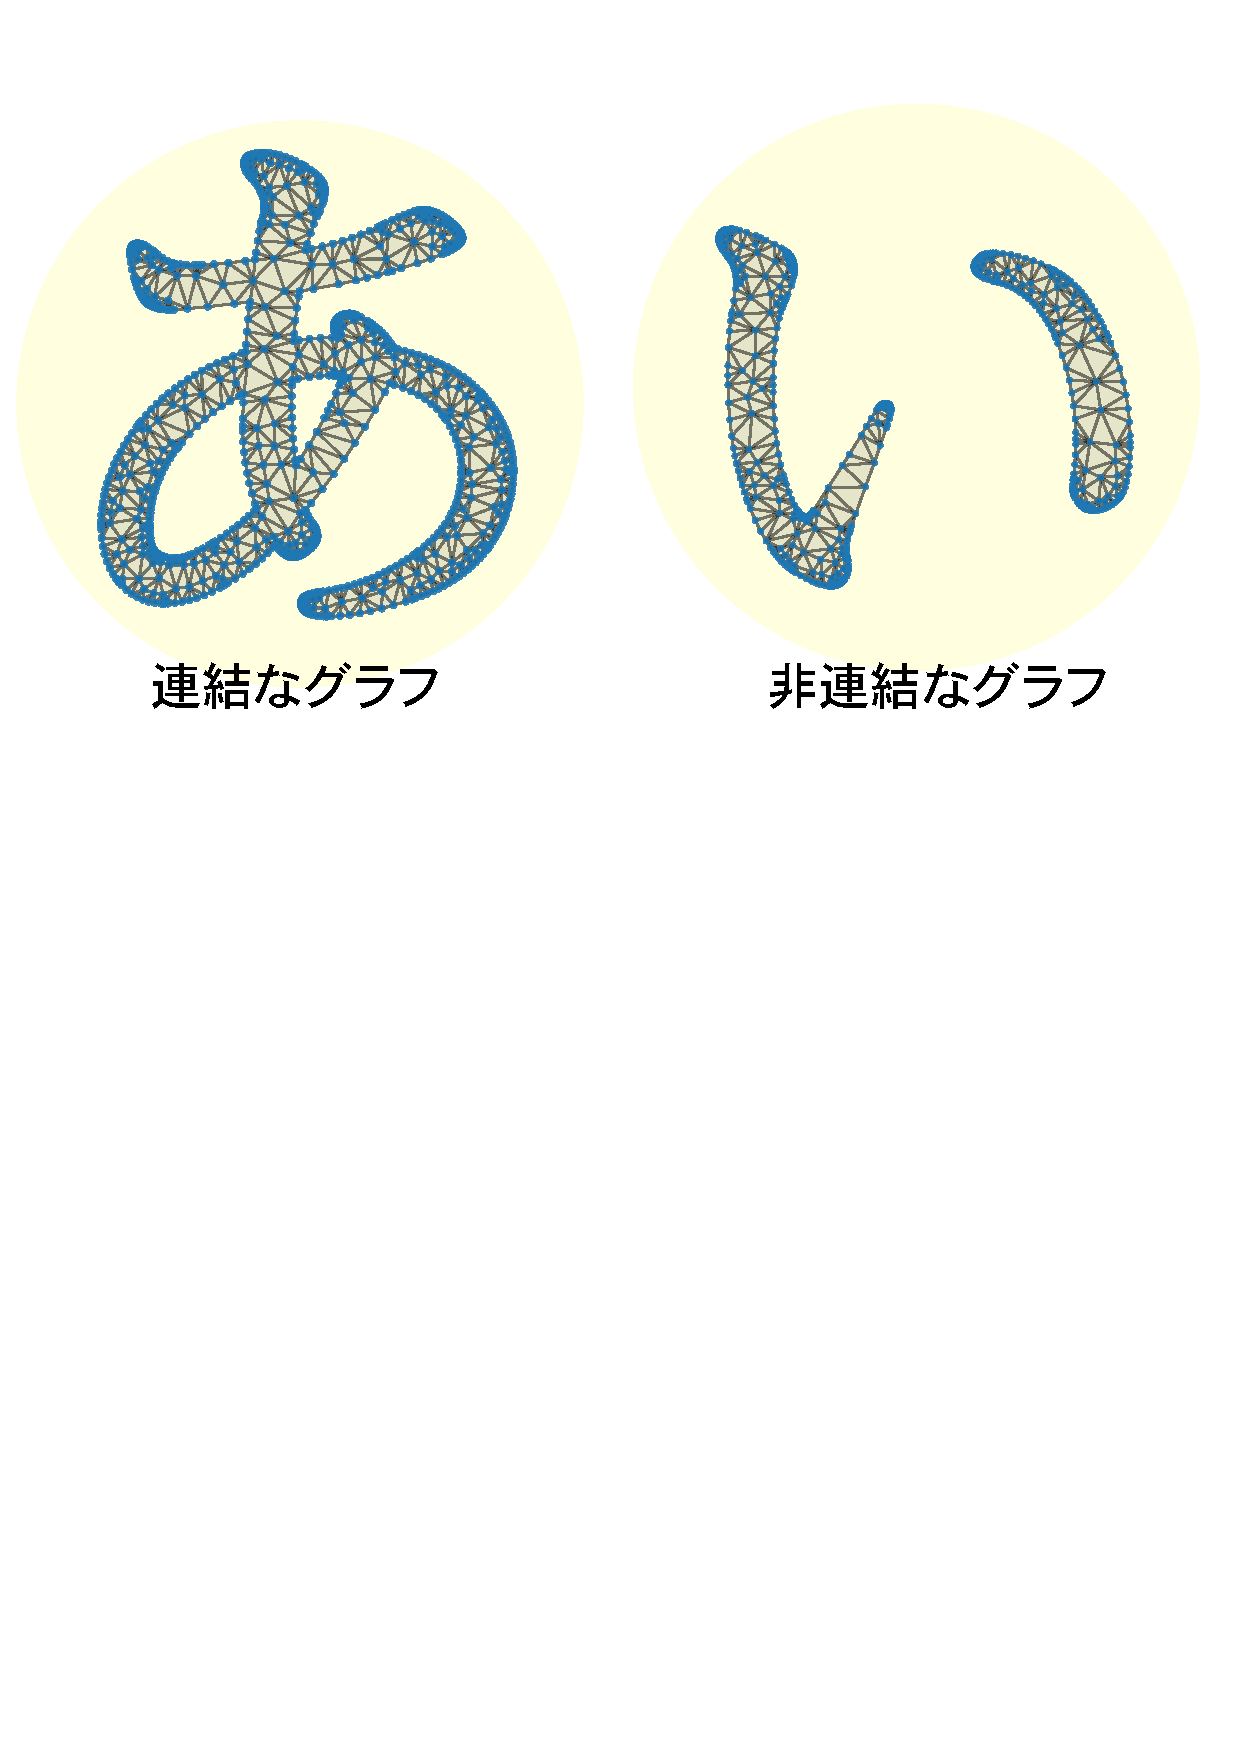
\includegraphics[width=0.29\textwidth]{figures/connect_ai.pdf}
%\end{figure}
\end{paracol}


境界条件には瑣末だが注意が必要である。
一つの頂点のみからなるグラフを\hlpink{自明なグラフ}という。
一般的に自明なグラフには連結・非連結の概念は導入されない。
ただ、自明な部分グラフとしての孤立点は$0$-連結成分として
他の成分とは区別されることがある。
いずれにしても、平面性判定において頂点数が$4$以下のグラフは
すべて平面的なので、自明なグラフは本質的に対象外にできる。
%グラフの平面性に関しては、
%以下の平面描画の定義から自明なグラフおよび孤立点は平面的になる。



%\paragraph{全域木}
%根付き木$T$は閉路を持たない連結なグラフで、根と呼ばれる頂点を一つ持つ。





\setcolumnwidth{0.75\textwidth, 0.25\textwidth}
\begin{paracol}{2}
\paragraph{平面描画と平面埋込み}
あるグラフ$G$の\hlpink{描画}$\Gamma$は、
各頂点$v$を平面${\mathbb R}^2$上の点$\Gamma(v)$へ、
各辺$(u, v)$を$\Gamma(u), \Gamma(v)$を端点とするジョルダン開曲線へ写像する関数である。
ジョルダン曲線は自己交差しない平面曲線で、
開という形容は端点が異なることを意味する。
\hlpink{平面描画}は二つの異なる辺の写像が交差しないことをいう。
ただし共通して持つ端点で接することは許される。
平面描画を持つグラフを\hlpink{平面的グラフ}という。
任意の平面描画は平面を連続な領域に部分分割する。
%集合$S$の部分分割$\{S_1, \ldots, S_k\}$は、$S = \bigcup_{S_i \in S} S_i$かつ、
%任意の$i, j~(i \neq j)$に関して$S_i \cap S_j = \varnothing$を満たす
%$S$の部分集合満の集まりである。
この部分領域を\hlpink{面}という。
また、非有界な領域を\hlpink{外面}という(右図$f_0$)。

あるグラフの描画は無限に存在するが、
等価な描画を類別することで表現方法は有限個に限定される。
ある描画が与えられたとき、
各頂点に関して接続する辺を例えば時計回りのような一定の基準に則って
順序付けた構造を\hlpink{組合せ埋込み}という。
二つの描画が等価であるというのは、等価な組合せ埋込みを持つことで、
すべての頂点の接続辺の回転順序が辞書式で一致することを意味する。
平面描画を与える組合せ埋込みを\hlpink{平面埋込み}という。



\switchcolumn
\centering
\vspace{0.5\intextsep}
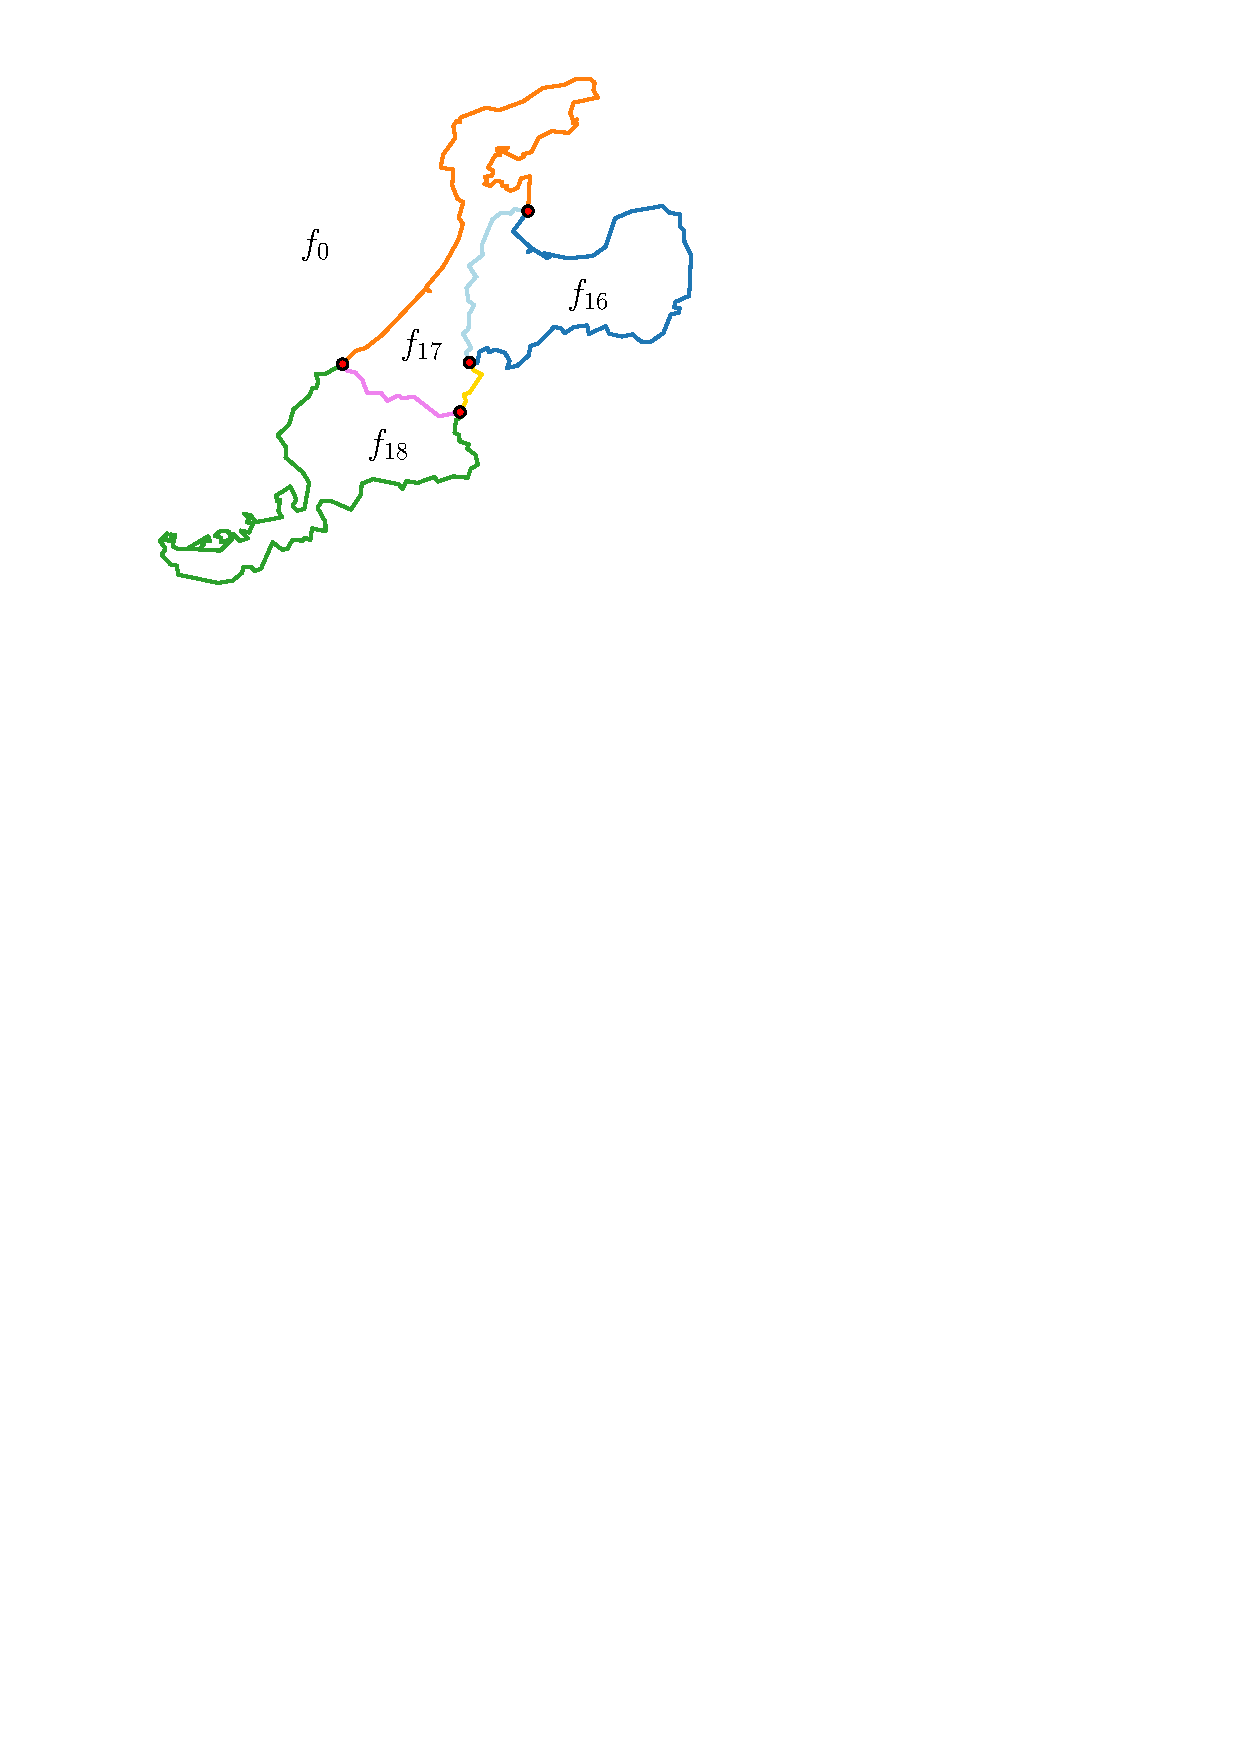
\includegraphics[width=0.24\textwidth]{figures/planar_drawing.pdf}

\vspace{1.\intextsep}
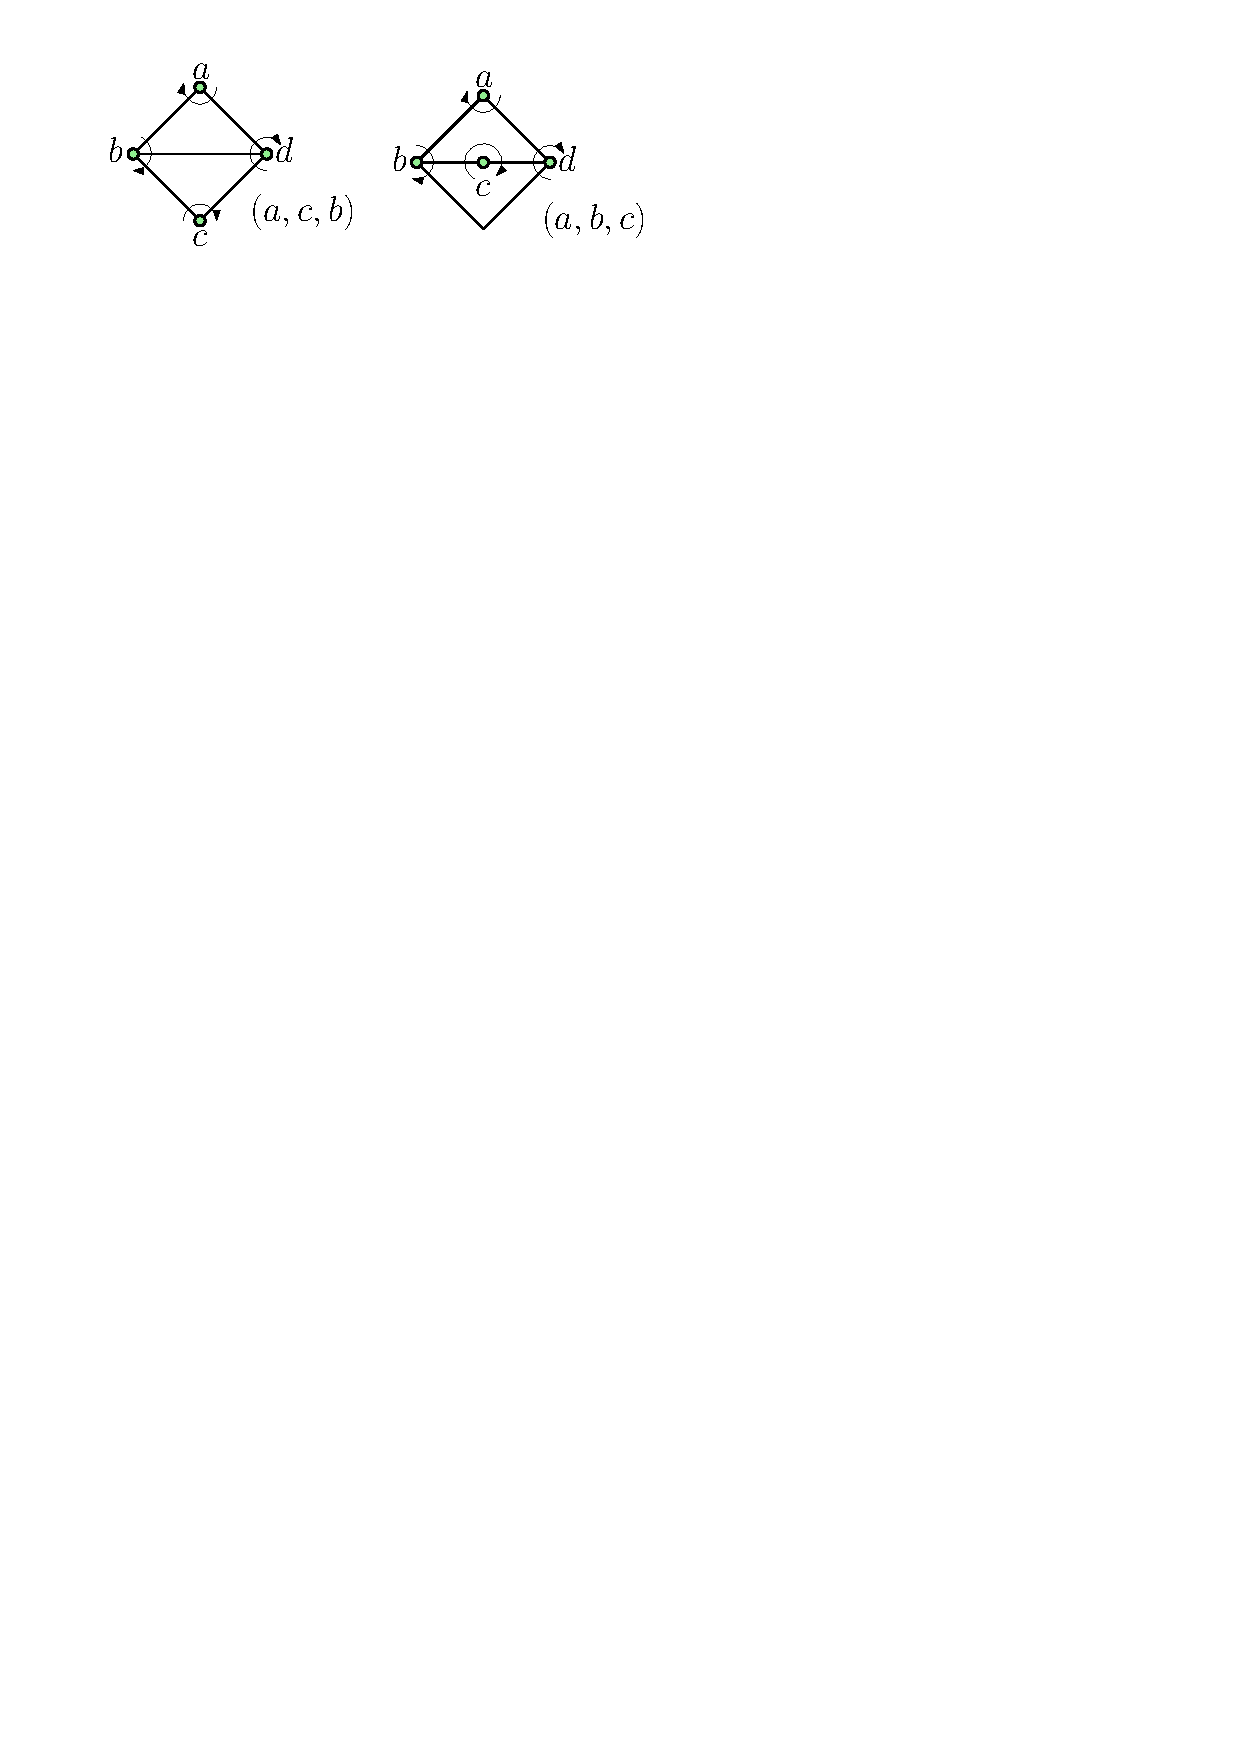
\includegraphics[width=0.24\textwidth]{figures/combinatorial_embedding.pdf}

\end{paracol}



\paragraph{極小性と極大性}
ある制約を満たす集合$S$が極小性を有するとは
$S$の要素を一つでも削除すると制約を満たさなくなることをいう。
同様に、極大性は$S$に要素を追加すると不成立になる飽和状態をいう。
例えば、辺集合が誘導する部分グラフの平面性に対する極小性と極大性を考える。
平面的なグラフから辺を削除しても平面性は損なわないが追加すると非平面的になり得るので
極大な平面的グラフを考えることができる。
極大な平面的グラフはその平面描画のすべての面が三辺で構成されるグラフとなる。
一方で極小な非平面的グラフはクラトフスキーグラフとなる
(クラトフスキーの\cref{thm:kuratowski})。

